\documentclass[article]{jss}
\usepackage[utf8]{inputenc}

\providecommand{\tightlist}{%
  \setlength{\itemsep}{0pt}\setlength{\parskip}{0pt}}

\author{
FirstName LastName\\University/Company \And Second Author\\Affiliation
}
\title{A Capitalized Title: Something about a Package \pkg{foo}}
\Keywords{keywords, not capitalized, \proglang{Java}}

\Abstract{
The abstract of the article.
}

\Plainauthor{FirstName LastName, Second Author}
\Plaintitle{A Capitalized Title: Something about a Package foo}
\Shorttitle{\pkg{foo}: A Capitalized Title}
\Plainkeywords{keywords, not capitalized, Java}

%% publication information
%% \Volume{50}
%% \Issue{9}
%% \Month{June}
%% \Year{2012}
\Submitdate{}
%% \Acceptdate{2012-06-04}

\Address{
    FirstName LastName\\
  University/Company\\
  First line Second line\\
  E-mail: \href{mailto:name@company.com}{\nolinkurl{name@company.com}}\\
  URL: \url{http://rstudio.com}\\~\\
    }

\usepackage{amsmath}

\begin{document}

\section{Introduction}\label{introduction}

This template demonstrates some of the basic latex you'll need to know
to create a JSS article.

\subsection{Code formatting}\label{code-formatting}

Don't use markdown, instead use the more precise latex commands:

\begin{itemize}
\tightlist
\item
  \proglang{Java}
\item
  \pkg{plyr}
\item
  \code{print("abc")}
\end{itemize}

\section{R code}\label{r-code}

Can be inserted in regular R markdown blocks.

\begin{CodeChunk}
\begin{CodeInput}
x <- 1:10
x
\end{CodeInput}
\begin{CodeOutput}
 [1]  1  2  3  4  5  6  7  8  9 10
\end{CodeOutput}
\end{CodeChunk}

\begin{CodeChunk}
\begin{CodeInput}
summary(iris)
\end{CodeInput}
\begin{CodeOutput}
  Sepal.Length    Sepal.Width     Petal.Length    Petal.Width   
 Min.   :4.300   Min.   :2.000   Min.   :1.000   Min.   :0.100  
 1st Qu.:5.100   1st Qu.:2.800   1st Qu.:1.600   1st Qu.:0.300  
 Median :5.800   Median :3.000   Median :4.350   Median :1.300  
 Mean   :5.843   Mean   :3.057   Mean   :3.758   Mean   :1.199  
 3rd Qu.:6.400   3rd Qu.:3.300   3rd Qu.:5.100   3rd Qu.:1.800  
 Max.   :7.900   Max.   :4.400   Max.   :6.900   Max.   :2.500  
       Species  
 setosa    :50  
 versicolor:50  
 virginica :50  
                
                
                
\end{CodeOutput}
\end{CodeChunk}

\subsection{Including Plots}\label{including-plots}

You can also embed plots, for example:

\begin{CodeChunk}
\begin{CodeInput}
# plot(pressure)
library(ggplot2)
ggplot(pressure) +
  geom_point(aes(temperature, pressure))
\end{CodeInput}


\begin{center}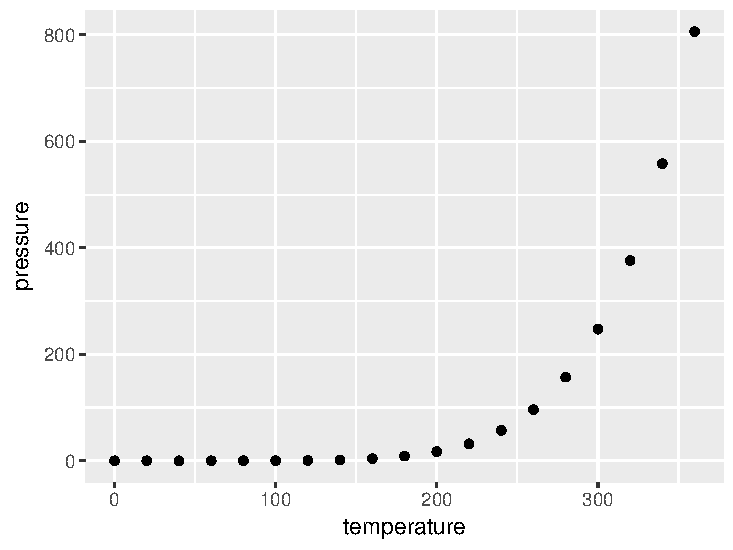
\includegraphics{Untitled_files/figure-latex/pressure-1} \end{center}

\end{CodeChunk}



\end{document}

